
\section{Exploiting Response Time Information\label{sec: ResponseTime}}

The response time is another major feature that has been previously exploited in Internet traffic analysis attacks. Like in the case of exploiting packet lengths, we would expect that the same attacks (as in the classical Internet setting) can be applied to 6LoWPAN traffic. Indeed, like in the previous section, we would expect that they will work even better because the accuracy of timing measurements can be greatly improved for 6LoWPAN traffic: this is because there are fewer noise sources in the traffic, the devices are physically close to each other and uses RF to communicate, the adversary can remove the RTT noises by measure the packets on the server side, and the performance of the constrained devices is low and hence gives a better resolution of the execution time.

\subsection{Distinguishing Different Sensors}
The first application of timing analysis that we describe is to distinguish between different sensors that are accessed on a device. For this purpose we set up an experiment on a CC2538, which has three on-board sensors: Vdd, temperature, and an Ambient Light Sensor (short ALS). We access these via CoAP\cite{rfc7252}, which is a protocol designed for constrained devices that provides an universal interface for accessing resources. CoAPs is the secure version which stands for CoAP with DTLS.

Due to the different physical characteristics of the sensors, there could be a variance of time that is required for reading the measurements. We investigated whether such variances could be observed through the packet response latency. If this was the case, then an adversary could learn the nature/purpose of sensors on a network by observing their response time. 

We thus set up an experiment on CC2538, using all three sensors from ``cc2538-demo". We used CoAP from the ``er-rest-example" in the Contiki OS source code, as there is no CoAPs implementation available. Although DTLS processing would definitely have an impact on the response latency, we argue that such impact would be independent to the sensors being accessed; hence similar result can be equally expected for CoAPs. We carefully controlled other factors, including URIs, data representation and code flow, to be uniform for all three sensors in order to guarantee a controlled environment.

\begin{table}
	\center
	\begin{tabular}{|c|c|c|}
	\hline
	& Average (ms) & Range(ms) \\ 
	\hline
	Vdd & 9.622 & [9.388, 10.318] \\ 
	\hline
	Temperature & 9.835 & [9.525, 10.318] \\ 
	\hline
	ALS & 11.651 & [11.338, 12.031] \\
	\hline
\end{tabular} 
	\caption{CoAP Response Latency for Sensor Readings on CC2538\label{CoapTiming}}
\end{table}

\Cref{CoapTiming} summarises the result. It shows that ALS takes about $2$ms longer and hence can be easily distinguished. Vdd and temperature have much more strongly overlapping distributions, and thus are more difficult to distinguish. Nevertheless these results confirm  our hypothesis: different sensors have different latencies and these leak through the response time. An adversary who is interested in finding out information about devices on a network might thus be able to match the (known) behaviour of `interesting' sensors to what they observe on the network. We remark that this could be useful even in the setting where the sensors transmit their data unencrypted: after all they might return only some reading without a unit of measurement; thus seeing their return data might not as such reveal their nature. 


\subsection{Distinguishing Different Devices}
%Gain hardware information.
%\begin{itemize}
%	\item Different hardware has different response latency against the same message.
%	\item For 802.15.4: Requires additional information. Can be satisfied by the previous ICMP attack.
%	\item For DTLS: No requirement. The adversary can actively send a message, e.g. PING.
%\end{itemize}

As we observed before, different devices have different underlying hardware and thus different computational power. This implies that there could be the potential that different devices take different amounts of time to process the same message. Because ICMP messages are standardised, they are particularly suitable for this purpose. Among the different ICMP messages, PING is especially ideal for two reasons: 
\begin{enumerate}
	\item It is mandatory in the ICMP standard.
	\item It only swaps the source and destination address of the packet; thus minimises different code path in protocol processing.
\end{enumerate}

\begin{table}
	\center
	\begin{tabular}{|c|c|c|}
	\hline
			& CC2538	& TelosB \\ 
	\hline
	Average(ms)	& 9.56		& 17.03 \\ 
	\hline
	Range(ms)	& [9.16, 10.06]	& [16.49, 17.68]	\\
	\hline
\end{tabular}

	\caption{PING Response Latency\label{PingResponse}}
\end{table}

\Cref{PingResponse} shows the PING response latency on CC2538 and TelosB. The result confirms that these devices can be distinguished by PING response latency.


\subsection{Distinguishing Programs}
%Fingerprints the code running on a device, which leads to plaintext recovery.
%\begin{itemize}
%	\item Theory explained in \Cref{FingerprintTheory}.
%	\item Requirement: needs to actively send messages. Any Request/Response protocol works, such as PING, DTLS Heartbeat, CoAP PING, etc. 
%	\item Not for 802.15.4: adversary can't join the network.
%	\item For DTLS: PING is available and confirmed. DTLS Heartbeat should work if supported.
%\end{itemize}

We remarked before that the functionality of a sensor is potentially valuable information. For instance some sensors might be predominantly passive, e.g. they might read the temperature and report it back periodically, whereas some sensors might control something upon receiving commands. Thus knowing the functionality enables an adversary to make (more) sense of the observed traffic in the network. This could be done if a `fingerprint' could be produced for different programs. From an adversary's perspective a positive result would imply that they could `fingerprint' products which are on the market and thus use this information to infer what program is running on a target device.

% program executing on the target is a valuable information in aspect of security and privacy, as it determines functionality of a device and therefore the contents of encrypted packets associated. For instance, knowing a target being an actuator that controls an air conditioner immediately suggests a packet directed to it might  be a controlling command.

%Our study shows that the response time of packets could also be exploited to reveal information of the program target is executing. To be more specifically, an adversary can collect ``fingerprints'', which we explain in the following section, from products available on the market and then use this information to breach the program running on a target device.


%How it works
To illustrate why this might work, we now look at \Cref{FingerprintTheory}. It illustrates two sensors receiving the same service request. In our example, at the time of receiving the request, Sensor Node 1 was idle and hence responded immediately, whilst Sensor Node 2 postponed the request for reading a sensor. Clearly, the response time on Sensor Node 2 would appear longer than that of Sensor Node 1.

\begin{figure}
	\center
	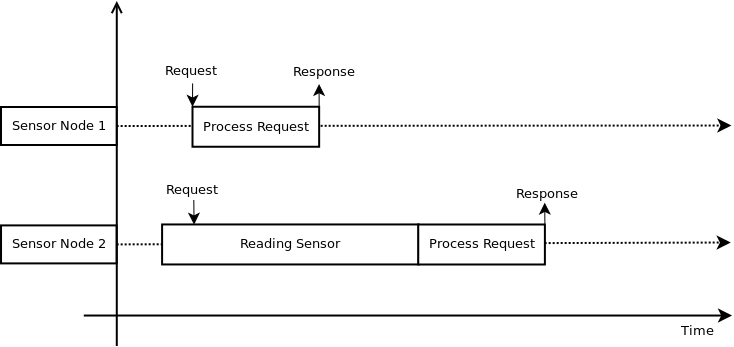
\includegraphics[width=\textwidth]{fig/PingProbe_Theory.png}
	\caption{Variations in Response Time\label{FingerprintTheory}}
\end{figure}

In real life, most sensors are programmed in a loop; therefore the same code fragments are repeated through the life time of a sensor. Each code fragment takes different time to execute and hence the response times vary. This behaviour could be statistically analysed and the resulting distribution could be stored as a `fingerprint' .


For this fingerprinting scenario, we must assume the adversary has the pre-knowledge of potential programs and can fingerprint them (or that they have access to a database that contains this information). To identify an unknown program running on target sensor, the adversary collects a new fingerprint and then matches it to available fingerprints. Clearly, to effectively launch the attack, the adversary needs to be able to send the request to a targeted sensor (requests with short predictable processing time are preferable as they induce less noise). 

In practice, the request can be instantiated by several messages defined in the sensor network protocols. PING is exceptionally ideal as it is mandatory in the ICMP standard\cite{rfc4433} and has only negligible computation. Other options but not excluded are Heartbeat in DTLS\cite{rfc6520}, Reset in CoAP\cite{rfc7252}, etc.

\subsubsection{Extracting Fingerprints}
We explored the feasibility of fingerprinting programs on an CC2538 running Contiki OS by using the PING command.

\Cref{ExamplePri} shows an example of captured packets. Contiki MAC\cite{ContikiMAC} sends duplicated PING requests. The response time, which refers to PING Response Interval, PRI, is defined to be the time between a PING response and its last paired request. The highlighted Packets 205 and 203 shows such an example.

\begin{figure}[!h]
	\centering
	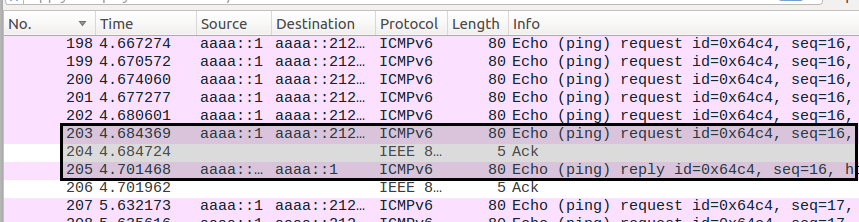
\includegraphics[width=\textwidth]{fig/PRI_hl.png}
	\caption{Example PRI\label{ExamplePri}}
\end{figure}

%Since the attack extracts the information contained in the extended response time of a specific request, the first problem is to see whether such extended response time can be filtered from normal ones. 

\Cref{HelloworldPriNormal} shows the histogram of PRIs collected on the ``helloworld'' example from Contiki OS. Values $\geq$12ms are collected at 12ms. The result shows that most PRIs are clustered around 9.5ms which consists with our result in \Cref{PingResponse}. The majority, roughly ranged [9.0, 10.3]ms, corresponds to the usual response time as depicted by Sensor Node 1 in \Cref{FingerprintTheory}. 

\begin{figure}[!h]
	\centering
	\begin{subfigure}{0.45\textwidth}
		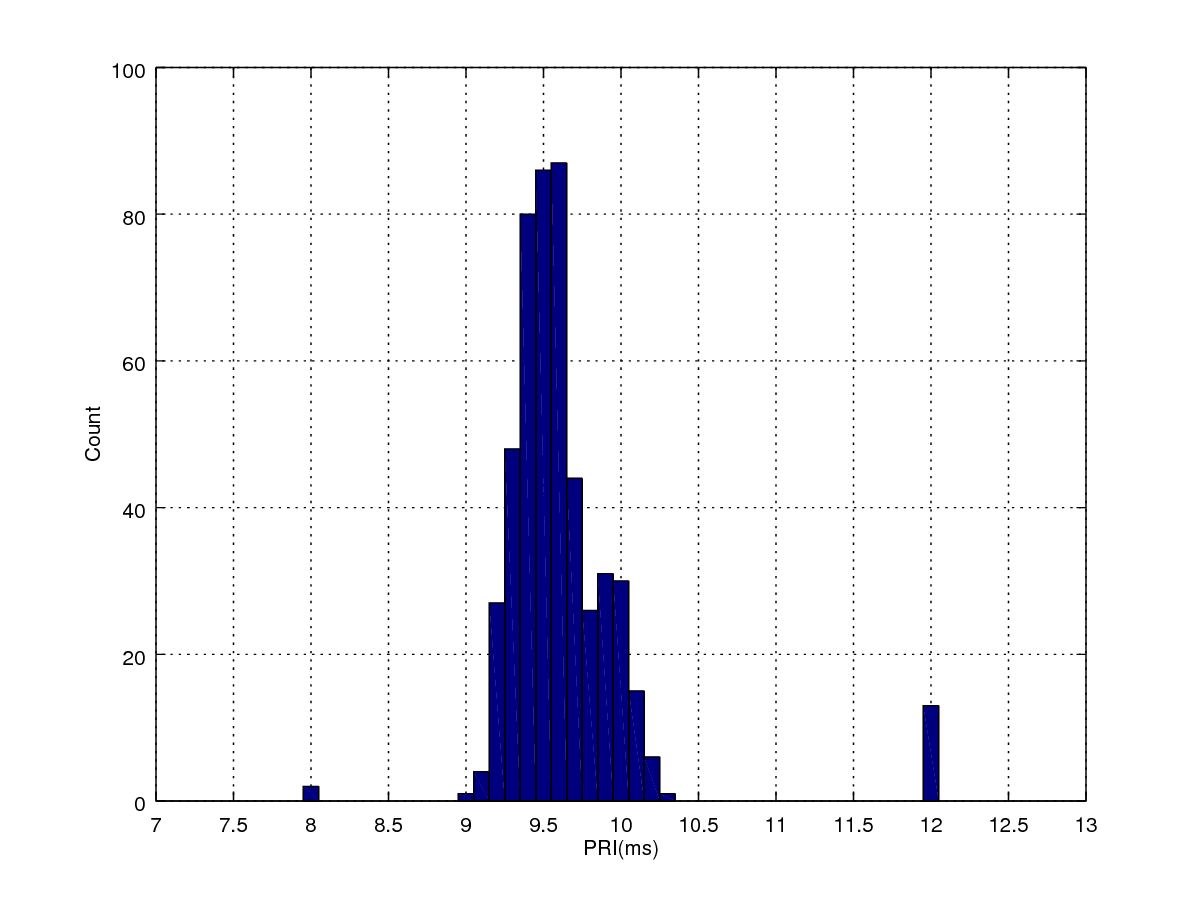
\includegraphics[width=\textwidth]{fig/helloworld_cc2538.png}
		\caption{PRIs of helloworld\label{HelloworldPriNormal}}
	\end{subfigure}
	\begin{subfigure}{0.45\textwidth}
		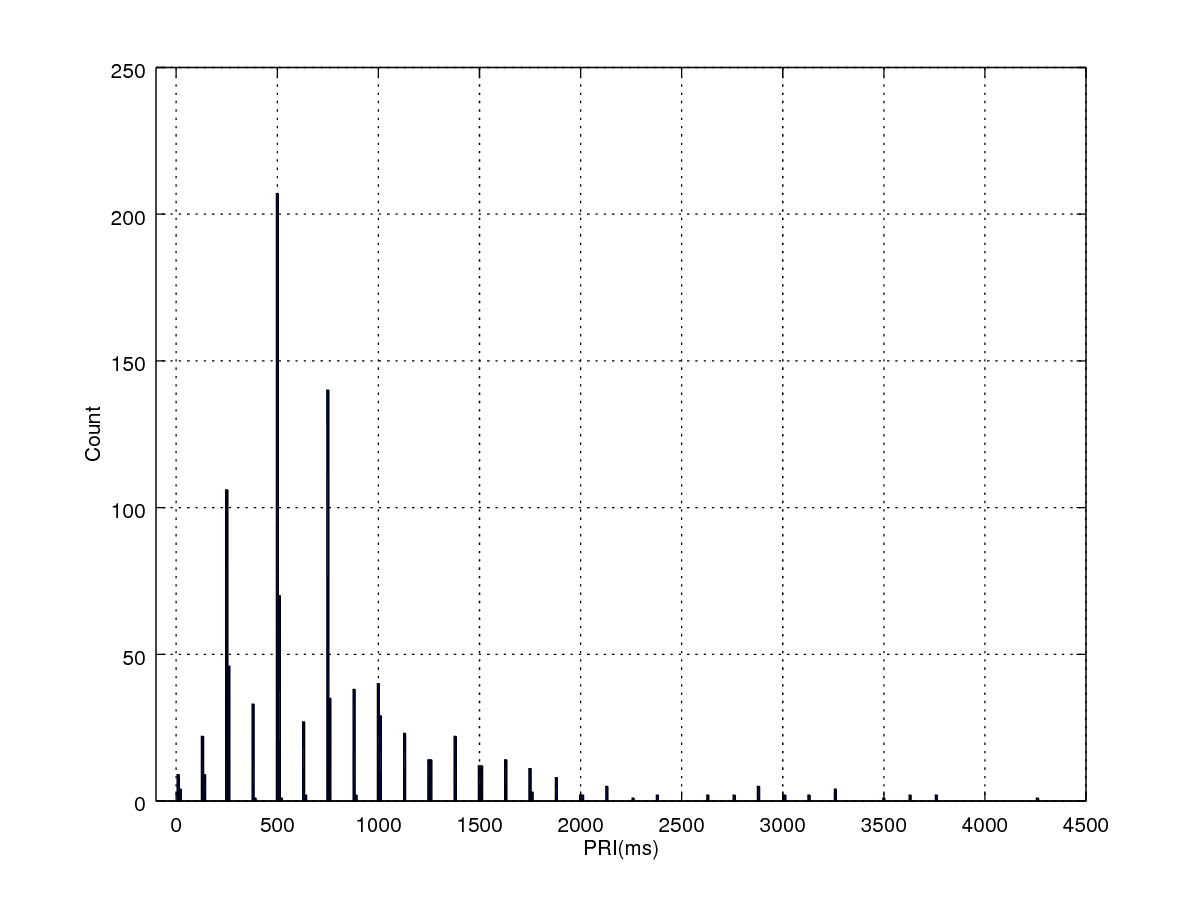
\includegraphics[width=\textwidth]{fig/helloworld_cc2538_outlier.png}
		\caption{PRIs outliers of helloworld\label{HelloworldPriOutliers}}
	\end{subfigure}
	\caption{helloworld PRIs\label{HelloworldPri}}
\end{figure}

We further plotted the upper outliers, mostly ranged [12, 2000]ms, in \Cref{HelloworldPriOutliers}. Unfortunately we do not have a solution to investigate the exact cause of such delay, as we were unable to control the code execution that requires environmental interaction within a timing critical context. Nevertheless, we suppose these outliers correspond to the extended response time as depicted by Sensor Node 2 in \Cref{FingerprintTheory}. The distribution described by \Cref{HelloworldPriOutliers} is the fingerprint of the ``helloworld'' example.

The result in \Cref{HelloworldPri} shows a clear gap between the usual PRIs and extended PRIs. In fact other applications we experimented also showed the same property. This implies that an adversary can easily draw a threshold by observing the whole PRI distribution and then filter out the fingerprint. In our experiments the threshold is set to 12ms but any other values within the gap would also work. 

We collected the fingerprints for three programs taken from the Contiki OS examples:
\begin{description}
	\item[broadcast] This program periodically broadcasts a constant message.
	
	\item[powertrace] This program records the power consumption and broadcasts a constant message.
	
	\item[Sensorpayload] This program is based on the ``er-rest-example'' embedded together with sensor accesses taken from ``cc2538-demo''. It captures a real case scenario where three different sensors, namely Temperature, Vdd and ALS, are being accessed through CoAP.
\end{description}

Specifically for ``Sensorpayload'' we collected fingerprints for 8 different scenarios where different sensors are being accessed. For each program we independently collected 2 fingerprints for comparison.

\Cref{FingerprintApps} summarises the total 20 fingerprints we collected for the experiment.

\subsubsection{Fingerprint Matching}
%Comparing the distribution.

During the experiments we realised that most of the fingerprints do not adhere to common distributions; therefore we used a non parametric test, the Kolmogorov-Smirnov Distance\cite{KsTest}, as our test statistic. This is a well understood statistic with previous uses in side channel analysis\cite{KsDistanceDistinguisher}. \Cref{ksdistances} summarises the relative KS distances computed on each pair of fingerprints in our experiments.

Although fingerprints collected on the same application were rejected by the Kolmogorov-Smirnov Test, we noticed that their KS distance tends to be smaller comparing to fingerprints collected on different programs, as the \textbf{bold} cells marked in \Cref{ksdistances}. 

By adapting our distinguisher to utilise the minimum KS distance, we were able to identify 13 out of 20 fingerprints successfully. The `overlapping' fingerprints are mainly due to the ``Sensorpayload'' program, which access different sensors, but otherwise has identical program code. Thus we did expect that the different instantiations of it would lead to very similar fingerprints. 
